\documentclass[smallextended]{svjour3}
\usepackage{fix-cm}
\usepackage[UTF8,fontset=windows]{ctex}
\setmainfont{Times New Roman}
\usepackage{amsmath,amssymb,graphicx,booktabs,tabularx,url}
\usepackage{placeins}
\usepackage[numbers,sort&compress]{natbib}
\usepackage[hidelinks]{hyperref}
\journalname{Computing（中文阅读译稿）}
\smartqed
\setlength{\emergencystretch}{2em}
\newcommand{\CollegePRDelta}{-0.90780}
\newcommand{\CollegePRLoss}{9.01}
\newcommand{\CollegePRSaving}{86.44}
\newcommand{\CollegePRfiveDelta}{-0.43094}
\newcommand{\CollegePRfiveLoss}{4.28}
\newcommand{\CollegePRfiveSaving}{82.83}
\newcommand{\CollegeDegreeDelta}{0.00000}
\newcommand{\CollegeDegreeLoss}{0.00}
\newcommand{\CollegeDegreeSaving}{86.59}
\newcommand{\GrqcPRDelta}{-0.25082}
\newcommand{\GrqcPRLoss}{5.07}
\newcommand{\GrqcPRSaving}{92.70}
\newcommand{\GrqcPRfiveDelta}{0.00000}
\newcommand{\GrqcPRfiveLoss}{0.00}
\newcommand{\GrqcPRfiveSaving}{88.14}
\newcommand{\GrqcDegreeDelta}{0.00000}
\newcommand{\GrqcDegreeLoss}{0.00}
\newcommand{\GrqcDegreeSaving}{92.77}
\newcommand{\WikiPRDelta}{-40.69334}
\newcommand{\WikiPRLoss}{73.01}
\newcommand{\WikiPRSaving}{96.42}
\newcommand{\WikiPRfiveDelta}{-13.53012}
\newcommand{\WikiPRfiveLoss}{24.28}
\newcommand{\WikiPRfiveSaving}{91.98}
\newcommand{\WikiDegreeDelta}{0.00000}
\newcommand{\WikiDegreeLoss}{0.00}
\newcommand{\WikiDegreeSaving}{96.26}

\begin{document}
\def\abstractname{摘要}\def\keywordname{\textbf{关键词}}\def\figurename{图}\def\tablename{表}\def\refname{参考文献}
\title{候选受限影响力最大化的评价：选择预算与排名精度的影响}
\titlerunning{候选受限影响力最大化的评价}
\author{\mbox{Jiayue Sun} \and \mbox{Binbin Yong} \and \mbox{Junjie An} \and \mbox{Tianyu Bo} \and \mbox{Shuai Li}}
\authorrunning{Jiayue Sun et al.}
\institute{Jiayue Sun \at 兰州大学人工智能学院，中国兰州，730000
\and Binbin Yong（通讯作者）\at 兰州大学信息科学与工程学院，中国兰州，730000 \\
\email{yongbb14@lzu.edu.cn}
\and Junjie An, Tianyu Bo 和 Shuai Li \at 兰州大学，中国兰州}
\date{}
\maketitle

\begin{abstract}
候选限制将贪心搜索的范围缩小到排名靠前的少数节点，从而加快影响力最大化求解。通常用全候选贪心结果评价这种限制的质量，但全候选参照本身是在有限个传播世界上优化得到的，进入受限候选池的节点也取决于排名的求解精度。本文考察选择预算和排名精度如何影响这一比较。全候选方法与受限方法使用相同的传播图、选择世界和同分规则，再用10,000个独立世界评估各自选出的种子集合。在三个SNAP网络的独立级联实验中，ca-GrQc上的PageRank-4k在80个选择世界下的增量传播量平均高于全候选参照5.6\%，在1,280个世界下则低于参照5.1\%。在事后分析中，将PageRank容差从$10^{-6}$收紧到$10^{-12}$后，20个候选节点中有两个发生替换，受限方法在三个预算下的平均传播量均高于参照。在四张接触图上，预算从1,280增至5,120个世界时，40个参照集合中有16个发生变化，但全部配对的平均传播量仅增加0.011个节点。在1,280个世界下，含20个节点的度候选池复现了全部15条参照种子序列，相对全候选穷举搜索节省超过98\%的选择时间；相同大小的PageRank池则损失了5--73\%的增量传播量。评价候选限制时，应报告哪些节点进入候选池，并在独立世界上测量最终种子集合的传播量。
\keywords{影响力最大化 \and 蒙特卡洛模拟 \and 候选限制 \and 评价方法 \and 可复现性}
\end{abstract}

\section{引言}
影响力最大化要求在给定传播模型下选取$k$个种子节点，使期望传播量最大\cite{ref1}。这类定向播种问题的一个例子是在社交网络上选择最初的采纳者。贪心算法逐轮加入估计边际收益最大的节点。每次估计都需要蒙特卡洛模拟，计算成本随节点数和采样世界数增加。惰性求值、复用采样结果和基于采样的求解器分别从不同环节降低成本\cite{ref7,ref8,ref2}。候选限制的做法更直接：先用度或PageRank等计算成本较低的指标排名，再让贪心算法只搜索前$q$个节点。是否值得缩小搜索范围，取决于节省了多少计算，以及保留了多少传播量。

通常以全候选贪心结果为固定基准来衡量这一权衡。然而，参照本身也是采样计算的产物。全候选搜索与受限搜索都在$W$个采样世界上优化估计目标；增加$W$可能改变任一方法的种子，二者的差值反映两侧的共同变化。另一个变化来源出现得更早，即候选池的构建。PageRank迭代到有限容差便停止；若截断位置附近的分数接近，微小的数值变化就可能替换边界处的候选节点。仅看种子集合是否一致难以区分这些影响，因为不同集合可能触达几乎相同数量的节点。

本文采用配对设计比较全候选与受限贪心选择（图~\ref{fig:evaluation-mechanism}）。两种搜索共享传播图、选择世界的嵌套前缀及同分规则，差别在于哪些节点有资格成为种子。随后在另一组10,000个世界上评估每个种子集合，以节点数表示配对传播差值。我们考察三个问题：排名容差是否改变预算比较的结果，所选种子改变时传播量变化多少，以及在给定损失下各候选限制能节省多少选择时间。

主实验采用三个SNAP网络，分别是通信网络CollegeMsg、合作网络ca-GrQc和投票网络wiki-Vote。网络在查看种子集合和传播量之前选定。本项目前期研究了四张小规模接触图，本文以其结果为对照，考察先前观察能否延伸至较大的网络。排名容差比较是在主实验结果得到后加入的，作为事后分析单独报告。

本文的主要贡献如下。
\begin{enumerate}
\item[(1)] \textbf{我们发现，排名精度可以改变预算比较中观察到的优劣反转。}在ca-GrQc上，默认容差下PageRank-4k的平均传播量在$W=80$时高于全候选参照，在$W=320$与1,280时低于参照。收紧容差替换了20个候选中的两个，此时三个预算下的平均差值均为正（表~\ref{tab:precision-output}）。
\item[(2)] \textbf{我们分别测量种子集合变化及其对应的传播量变化。}独立世界上的配对评估显示，在接触图上，当$W$从1280增至5,120时，40个参照集合中有16个改变，全部配对的平均传播量仅增加0.011个节点，各配对的差值有正有负。
\item[(3)] \textbf{我们量化了缩小候选范围所节省的计算及其传播代价。}在$W=1280$时，Degree-4k复现了SNAP网络的全部15条参照种子序列，相对全候选穷举搜索节省98.4--99.7\%的选择时间。PageRank-4k未复现其中任何一条。在两个有向网络上，将PageRank池扩大到节点总数的5\%可缩小传播损失，但仍低于参照。
\end{enumerate}

\begin{figure}[t]
\centering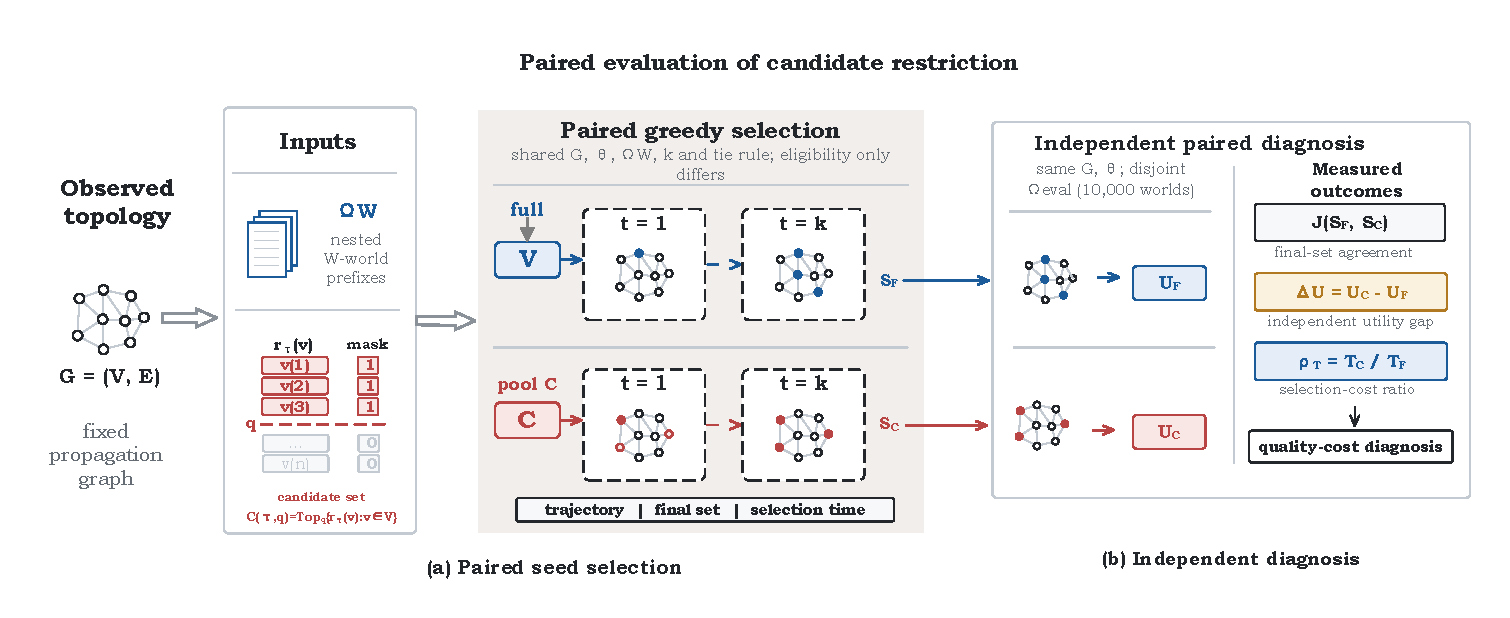
\includegraphics[width=\linewidth]{FigEvaluationMechanism.pdf}
\caption{配对评价设计。（a）全候选与受限贪心选择共享图、传播参数$\theta$、$W$个选择世界的嵌套前缀、种子预算$k$及同分规则。受限方法只搜索候选池$C(\tau,q)$，该池由容差$\tau$下排名最高的$q$个节点组成。（b）两个种子集合使用同一组$M=10{,}000$个评估世界，与选择世界分离。输出包括传播差值$\Delta U$（受限减全候选）、最终集合的Jaccard相似度$J$和选择时间比$\rho_T$。}\label{fig:evaluation-mechanism}
\end{figure}

\section{相关工作}
\paragraph{高效贪心选择。}Kempe等证明独立级联模型下的期望传播量具有单调性和次模性，由此得到贪心选择的近似保证\cite{ref1}。CELF利用次模性跳过不会改变当前选择的边际收益重算\cite{ref7}。StaticGreedy在整个搜索过程中固定一组采样结果，使所有候选在同一覆盖目标下评分\cite{ref8}。IMM以具有近似保证的采样求解器替代前向模拟\cite{ref2}。这些方法降低给定目标的优化成本。候选限制改变的是可行集合，传播效果取决于截断排名排除了哪些节点。本文固定模拟器和贪心规则，分别考察候选资格、选择预算或排名容差的变化。

\paragraph{影响力估计与种子搜索。}Rui等利用多层邻域估计影响力\cite{ref12}，Fan等用离散哈里斯鹰优化器搜索种子\cite{ref13}，Ko等提出的MONSTOR+可预测未见图上的传播量\cite{ref19}。这些方法各自提供估计器或搜索程序。本文考察排名的一项特定用途：只用排名决定贪心搜索可以选择哪些节点，传播和评估仍在完整图上运行。在这一用途下，可以通过候选池对全候选参照种子的覆盖情况来理解排名的表现。

\paragraph{影响力最大化方法的评价。}Li等综述了该领域的方法\cite{ref9}；Arora等对既有方法的传播效果和运行时间进行了基准比较\cite{ref16}。Yanchenko等梳理了时间网络上的问题定义\cite{ref11}，Aral与Dhillon研究了基于实证估计传播模型的影响力最大化\cite{ref15}。这些研究表明，算法比较需要结合传播模型、网络表示与评价协议。本文关注评价协议：当计算成本较低的搜索与采样得到的全候选参照比较时，观测差值如何随候选限制、选择预算及排名计算而变化？我们通过控制这些设置，在独立世界上测量相应的效用差异。

\section{研究方法}
我们在同一传播图上比较全候选与受限贪心选择。第~\ref{sec:paired}节定义选择目标和术语，第~\ref{sec:coupling}节说明选择世界和评估世界的构建，第~\ref{sec:cost}节说明成本测量方式。网络统计量与参数值见第~\ref{sec:experimental-setup}节。
\subsection{配对贪心选择}\label{sec:paired}
设$G=(V,E)$为有向传播图，$S$为大小为$k$的种子集合。在独立级联模型下，每个新激活节点有一次机会以概率$p$激活其每个尚未激活的出邻居。传播在$h$轮后停止。在随机世界$\omega$中，$f_h(S;\omega)$表示包括种子在内的激活节点总数。贪心选择采用采样目标
\begin{equation}
\widehat\sigma_W(S)=\frac{1}{W}\sum_{w=1}^{W}f_h(S;\omega_w).
\end{equation}
每一轮对所有尚未选中的合格节点$v$评分，并加入整数总和$W\widehat\sigma_W(S\cup\{v\})$最大的节点。直接比较整数总和可精确识别同分，再按原始节点ID的字典序打破平局。全候选选择使用$C=V$，受限选择使用候选池$C\subset V$。两者均在完整传播图上模拟。

本文将规定种子候选资格的规则称为\emph{方法}，如全候选选择、Degree-4k或PageRank-5\%。一次\emph{计算重复}使用各自的选择世界和评估世界，并以编号标识（SNAP网络为1101--1105）。一组\emph{配置}固定图、重复编号、选择预算$W$及随机世界的耦合方式。配置内各方法共享随机世界、种子预算$k$及同分规则。每个受限方法均与同一配置下的\emph{全候选参照}比较。

在预算扫描中，候选池固定。全候选参照和各受限方法在每个$W$下均使用同一嵌套前缀重新选择种子。因此，差值随$W$变化可能源于任一侧的搜索。排名容差$\tau$和候选池大小$q$与$W$分别控制。

度排名按不同出邻居的数量降序排列。PageRank在无权有向图上按NetworkX 3.5的默认设置计算：阻尼系数0.85，均匀个性化向量，按默认方式处理悬挂节点，容差$\tau=10^{-6}$，最多迭代100次\cite{networkxpr}。相邻两次迭代的分数向量之差的$L_1$范数小于$n\tau$时停止，其中$n=|V|$。分数相同时按节点ID的字典序排序。4k池取前$q=\min(n,4k)$个节点，5\%池取前$q=\lceil0.05n\rceil$个节点。事件加权度在CollegeMsg上统计发出的消息数，在无向接触图上统计各节点参与的保留接触记录数。每次保留的接触表示为一对互向弧，两个端点各计一条出向记录（Weighted-4k和Weighted-5\%）。作为基线，每张图的每次重复另抽取三个大小为$4k$的随机池，在不同预算和耦合方式下复用。

\subsection{世界耦合与独立评估}\label{sec:coupling}
主实验采用\emph{按步耦合}，每个随机抽样值由世界、传播步、源节点和目标节点共同索引。给定种子集合时，该耦合给出独立级联模型的传播量分布，但有限样本上的目标可能不单调：将中间节点设为种子会使其更早尝试激活出邻居，因使用了不同的随机数，最终传播量可能降低（反例见在线补充材料1）。为与早期实验可比，主实验沿用按步耦合，另设固定边对照。\emph{固定边耦合}在每个世界内对每条边只抽样一次，其采样目标为从$S$出发经过至多$h$条可传播边能触达的节点数，具有单调性和次模性。两种耦合都采用穷举贪心搜索，逐轮枚举尚未入选的合格节点。对固定边覆盖目标，CELF可以复用先前的边际收益作为上界；若在按步耦合目标下采用同一做法，则需要边际收益递减的保证。每个受限方法与自身耦合方式下的全候选参照比较。

选择世界按预算形成嵌套前缀：增加$W$时追加世界，并保留先前的抽样。对每张图、每次重复和每种耦合方式，评估使用$M=10{,}000$个与选择世界分离的世界。在SNAP实验和含520组配置的接触图扩展中，这些评估世界均跨方法、跨预算共享。图、重复编号与随机候选池抽样由不同的键区分。

设$S_C$为受限方法的种子集合，$S_F$为全候选参照种子集合。评估世界$i$上的配对差为$d_i=f_h(S_C;\eta_i)-f_h(S_F;\eta_i)$。两者均在相同$W$下选出；$d_i$为正表示受限方法传播量更大。图~\ref{fig:evaluation-mechanism}中的效用差为
\begin{equation}
\widehat\Delta=\frac{1}{M}\sum_{i=1}^{M}d_i,
\qquad \operatorname{SE}_{\rm MC}=s(d_i)/\sqrt M.
\end{equation}
区间$\widehat\Delta\pm1.96\operatorname{SE}_{\rm MC}$描述两个固定种子集合传播差值的蒙特卡洛不确定性。重复间标准差描述不同重复所选种子的变异，其中也包含评估噪声。对于随机池，在每次重复内先将三个池的逐世界评估向量取平均，再计算上述统计量。

与全候选参照的一致性通过有序种子序列是否相同、最终集合是否相同以及最终集合的Jaccard相似度报告，同时记录首次分歧的轮次。增量传播量为总传播量减去$k$个种子。受限方法的百分比损失为$-100\widehat\Delta/(\widehat\sigma_{\rm full}-k)$，其中$\widehat\sigma_{\rm full}$为同一次重复的$M$个评估世界上全候选参照的平均总传播量。损失为正表示受限集合触达的节点更少。先逐次重复计算损失，再取平均。

每张图分别对$W=1280$下预先指定的三项主要比较进行双侧配对符号检验，并在图内使用Holm校正。三项比较分别是Degree-4k、PageRank-4k、三个随机池的均值各自与全候选参照的比较。主要结果揭晓前，协议已规定这些比较。零差值单列报告，并从符号检验中排除。覆盖率、耦合与预算变化的分析采用描述性统计，计算重复反映给定网络上的计算变异。

\subsection{实现与成本测量}\label{sec:cost}
实现使用Numba，按配置和方法记录候选ID、种子选择顺序、各轮整数总分及逐世界评估值。复现与核验流程见在线补充材料1。

选择时间包括贪心搜索及候选ID的字典序排序；图准备、世界生成和评估分别计时。为估计预热进程中一次完整运行的成本，我们将文件解析、建图以及该方法的排名与建池成本（五次重复的中位数），加到已记录的选择世界准备、种子选择、评估世界准备及独立评估耗时上。该分项合计不含导入、即时编译、下载和输出写盘。

在重复编号1101、$W=320$时，以随机方法顺序重复计时五次，考察耗时变异。所有成本比较均以本实现的全候选穷举搜索为参照，PageRank使用默认容差。较严格容差仅用于质量分析。

\paragraph{AI工具使用。}OpenAI Codex协助完成了基础代码开发与文稿起草。作者对最终稿件承担责任。

\section{实验设置}\label{sec:experimental-setup}
主实验在三个SNAP网络上模拟独立级联传播，设置为$k=5$、$p=0.01$、$h=3$，并与本项目早期接触图研究的结果对照。

\paragraph{输入与输出。}每次运行输入处理后的网络及弧的方向、参数$k$、$p$、$h$、选择预算$W$和候选规则。排名容差$\tau$与截断位置$q$决定受限候选池，所有节点仍参与传播。选择阶段输出$k$个种子的有序序列及选择耗时。评估阶段输入最终集合和该次重复的$M$个评估世界，输出总传播量、增量传播量，以及与同预算全候选参照的配对差值。表~\ref{tab:primary}和表~\ref{tab:case}将这些输出与候选数量、原始节点ID对应列出。

\subsection{网络与预处理}
在查看种子集合及传播量之前，我们选定三种类型的SNAP网络\cite{snap}：CollegeMsg（通信）、ca-GrQc（合作）和wiki-Vote（投票）。表~\ref{tab:data}列出处理后的规模和候选覆盖率。所有弱连通分量均予以保留。
\begin{table}[htbp]
\caption{处理后的SNAP网络。弧表示有向传播边。4k占比为20个候选节点占全图节点数的比例，5\%候选池含$\lceil0.05n\rceil$个节点。}\label{tab:data}
\begin{tabular}{lrrrr}
\toprule
网络 & 节点数 & 弧数 & 4k占比 & 5\%池大小 \\
\midrule
CollegeMsg & 1,438 & 13,397 & 1.391\% & 72 \\
ca-GrQc & 5,241 & 28,968 & 0.382\% & 263 \\
wiki-Vote & 7,115 & 103,689 & 0.281\% & 356 \\
\bottomrule
\end{tabular}
\end{table}

CollegeMsg记录带时间戳的定向消息\cite{college}。沿用接触图研究的历史窗口，保留最早的65\%不同时间戳，即58,911个时间戳中的$\lfloor0.65\times58{,}911\rfloor=38{,}292$个，对应的截止Unix时间为1085640224。删除自发消息后，以保留的38,939个事件构建有向图，并按每个节点发出的消息数排名。同一对节点之间的重复消息合并为一条传播弧，但每条消息都计入发送者的消息数。所有弧使用统一的传播概率$p$。

ca-GrQc以合著关系连接作者\cite{grqc}。我们去除自环、合并重复节点对，并为每对节点添加互向弧。节点12295仅出现于自环，因而被去除，处理后得到5,241个节点，SNAP所列原始节点数为5,242。在wiki-Vote中，弧从投票者指向被投票者\cite{signed,links}。我们去除自环和重复弧，沿原方向模拟影响传播。两个静态数据集都没有事件计数，因而三个SNAP网络中只有CollegeMsg使用事件加权候选池。处理后CollegeMsg、ca-GrQc和wiki-Vote的弱连通分量数分别为2、354和24。原始节点ID以字符串保存，用字典序确定节点索引、排名同分及贪心选择同分的先后次序。原始与处理后文件的哈希见数据清单。

本项目前期使用四张含75--402个节点的接触图，来自工作场所、会议及肯尼亚农村的接触记录\cite{ref3,ref4,ref5,ref6}。初始研究包含42组配置，随后扩展为520组配置，接触图各有十次计算重复。扩展研究将选择预算提高至$W=5120$，考察$(p,h)$的四组局部参数变化、固定边采样、较大的种子预算$k=20$以及两个各含2,000个节点的固定合成图实例\cite{ref17,ref18}。参数比较中的默认设置复用预算扫描结果。接触图完整结果见在线补充材料1。

\subsection{主要实验设计与排名精度分析}
SNAP网络的设计见表~\ref{tab:settings}。主实验组合三张图、五次计算重复及三个选择预算$W\in\{80,320,1280\}$，共45组按步耦合配置。另设九组固定边配置，在$W=320$时使用重复编号1101--1103。每组均执行全候选、Degree-4k、PageRank-4k、Degree-5\%、PageRank-5\%及三个随机4k池的选择。CollegeMsg另含Weighted-4k和Weighted-5\%。每张图18组配置，共执行$18\times(10+8+8)=468$次方法运行。

\begin{table}[htbp]
\caption{SNAP网络的实验设置。}\label{tab:settings}
\begin{tabularx}{\linewidth}{lX}
\toprule
项目 & 设置 \\
\midrule
传播模型 & 独立级联；统一概率$p=0.01$；传播期限$h=3$；种子数$k=5$ \\
主要选择实验 & 按步耦合；$W\in\{80,320,1280\}$；重复编号1101--1105 \\
独立评估 & 每张图、每次重复及每种耦合使用$M=10{,}000$个评估世界，跨方法与预算共享 \\
候选池大小 & $4k=20$或$\lceil0.05n\rceil$；每次重复另设三个含20个节点的随机池 \\
固定边对照 & $W=320$；重复编号1101--1103 \\
默认PageRank & 阻尼系数0.85；$\tau=10^{-6}$；最多迭代100次 \\
严格容差PageRank（事后） & $\tau=10^{-12}$；最多迭代1,000次；在$10^{-14}$下候选成员相同 \\
重复计时 & 每种方法重复五次，运行顺序随机；重复编号1101，$W=320$ \\
\bottomrule
\end{tabularx}
\end{table}

排名精度分析在得到主要结果后加入。在原有五次重复上，以$\tau=10^{-12}$、最多1,000次迭代重新计算PageRank，并在各$W$下重做受限搜索；再使用相同的评估世界，与原同预算全候选参照比较。将容差进一步收紧至$\tau=10^{-14}$时，候选成员保持一致。两阶段分析过程见在线补充材料1。

\subsection{随机化、执行与可复现性}
所有随机抽样均由哈希键生成，以区分图、重复编号及选择和评估世界。提高$W$时只追加选择世界，不重抽已有前缀；同时核对选择与评估世界标识符没有交集。随机候选池使用独立的随机键，并在不同预算与耦合间复用。键的完整定义、世界标识符构造及哈希到随机数的映射见在线补充材料1的“可执行复现流程”。

实验在Windows上以单工作进程串行运行，使用Python 3.13.0、NumPy 2.3.3、NetworkX 3.5、SciPy 1.16.1及Numba 0.68.0，BLAS和OpenMP均限用一个线程。主机有20个物理核心和约32 GiB内存。计时前预热即时编译器，并随机排列方法运行次序以避免系统性的顺序效应。

\section{研究结果}
\subsection{预算比较对PageRank容差的敏感性（事后分析）}
在ca-GrQc上，PageRank-4k与参照的比较方向随PageRank求解容差而变（图~\ref{fig:precision-budget}、表~\ref{tab:precision-output}）。使用默认容差时，在$W=80$下，PageRank-4k的增量传播量平均高于全候选参照5.6\%；在$W=320$和1,280时，分别低于参照2.5\%和5.1\%。使用严格容差时，三个预算下的均值分别高于参照11.3\%、3.0\%和0.5\%。这是事后分析，各平均差值的绝对值至多为0.49个节点；作为对照，$W=1280$时参照的增量传播量为4.9个节点。差值的重复间标准差为0.08--0.27个节点。

在候选池边界处，收紧容差使节点1488和19865退出20节点池，17655和6610进入。在每个预算下，五次重复的最终种子集合均因此改变。即使固定严格容差候选池，选择预算仍影响结果：从80增至320个世界时，五次重复中有三次改变种子集合；从320增至1,280时，有两次改变。在$W=1280$时，严格容差下的平均差值为$+0.026$个节点，各次重复的差值在$-0.041$至$+0.179$之间，正负均有。

在两个有向网络上，收紧容差后PageRank-4k仍有损失。在CollegeMsg上，两种容差得到相同的候选池、种子和评估结果，三个预算下的损失分别为9.3\%、8.5\%和9.0\%。在wiki-Vote上有一个候选节点被替换，但严格容差下各预算的损失仍约为74\%。

\begin{table}[htbp]
\caption{ca-GrQc上默认容差（$\tau=10^{-6}$）与严格容差（$\tau=10^{-12}$）的PageRank-4k结果。差值为受限方法减同预算全候选参照的传播量，单位为节点，报告五次重复的均值，括号内为重复间标准差。“集合改变”指两种容差选出不同最终集合的重复次数。}\label{tab:precision-output}
\centering\begin{tabular}{rrrr}\toprule
$W$ & 默认差值（SD） & 严格差值（SD） & 集合改变 \\ \midrule
80 & +0.23606 (0.27402) & +0.48570 (0.24999) & 5/5 \\
320 & -0.12632 (0.18077) & +0.13804 (0.17387) & 5/5 \\
1280 & -0.25082 (0.07636) & +0.02608 (0.09155) & 5/5 \\
\bottomrule\end{tabular}
\end{table}

\begin{figure}[t]
\centering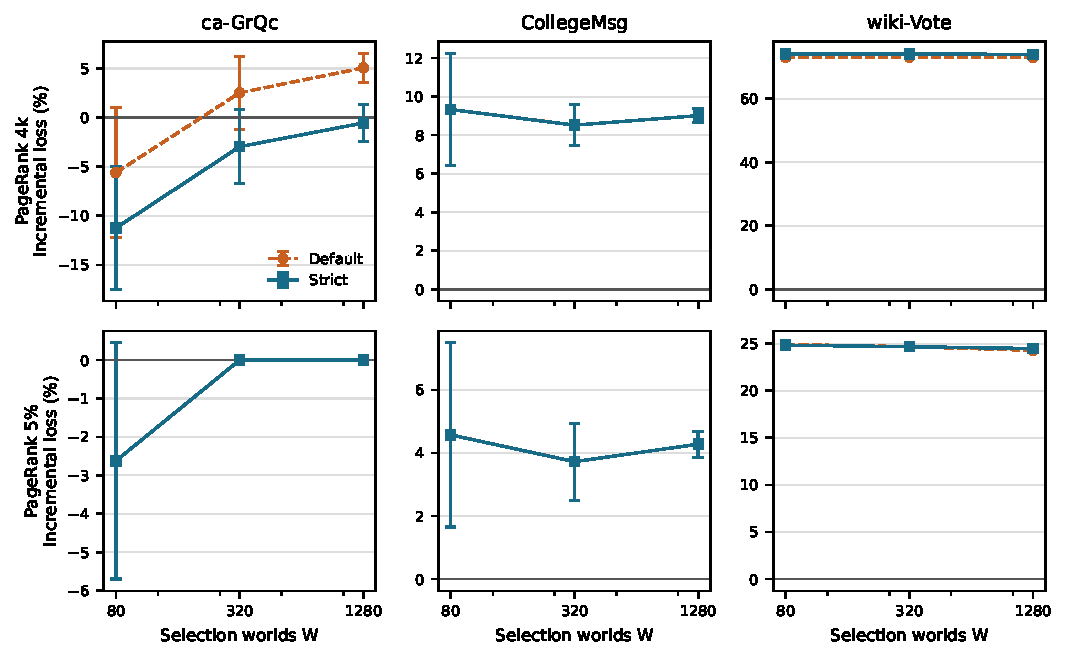
\includegraphics[width=\linewidth]{Fig4.pdf}
\caption{与同预算全候选参照相比，两种PageRank候选池在默认（$\tau=10^{-6}$）及严格（$\tau=10^{-12}$）容差下的增量传播损失。上排为4k池，下排为5\%池。点为五次重复的均值，误差线为重复间标准差。正损失表示受限种子集合触达的节点较少。在ca-GrQc上，默认容差的4k池损失随预算改变符号，严格容差下均小于零。CollegeMsg和wiki-Vote在两种容差下均有损失。}\label{fig:precision-budget}
\end{figure}

\subsection{参照集合改变时的传播量变化}
随$W$提高，全候选参照的种子集合常会改变，但对应传播量的变化较小，且有正有负（图~\ref{fig:transitions}）。从$W=320$增至1,280时，ca-GrQc的五个参照集合全部改变，传播量平均变化$+0.127$个节点，范围为$-0.027$至$+0.241$。CollegeMsg有一个集合改变，全部五次重复的平均传播量增加0.053个节点。wiki-Vote上部分种子顺序改变，最终集合均相同；由于传播只取决于集合，各次配对差均恰为零。在六个集合改变的比较中，四个差值的95\%蒙特卡洛区间完全高于零，另两个区间均来自ca-GrQc，包含零。

在更高预算下，接触图研究也观察到类似结果。按步耦合中，$W$从1280增至5,120时，40个参照集合有16个改变，传播量平均变化$+0.011$个节点（范围$-0.038$至$+0.118$）。固定边耦合中，$W$从320增至1,280时，40个集合有29个改变，传播量平均变化$+0.062$个节点（范围$-0.011$至$+0.257$）。每个预算比较在各自耦合方式内共享评估世界，两种对照覆盖的预算区间不同。
\begin{figure}[t]
\centering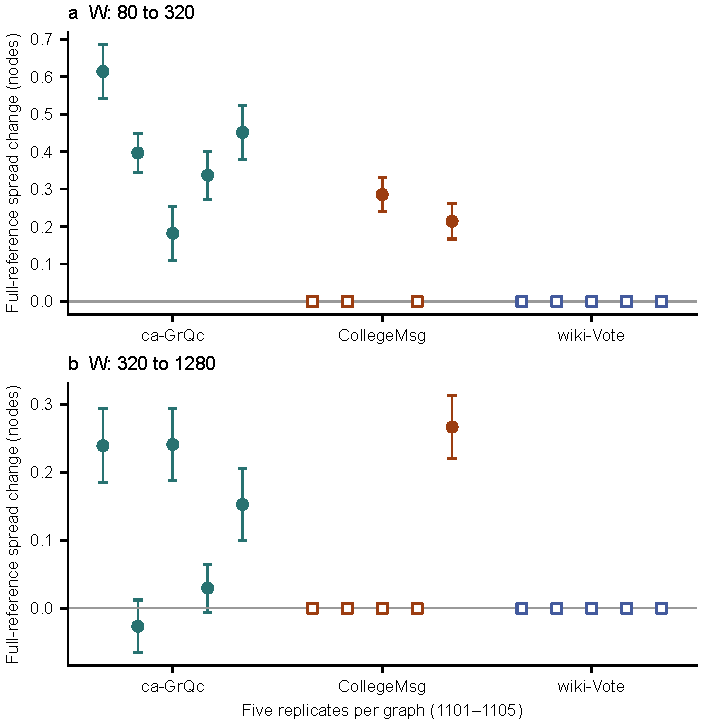
\includegraphics[width=\linewidth]{Fig2.pdf}
\caption{SNAP网络各次重复中全候选参照传播量的变化，高预算减低预算。（a）$W$从80增至320；（b）$W$从320增至1,280。各图内从左至右为重复编号1101--1105。实心圆表示最终集合改变，空心方块表示最终集合相同。误差线为根据10,000个配对评估世界计算的未经校正的95\%蒙特卡洛区间。两个面板的纵轴尺度不同。}\label{fig:transitions}
\end{figure}

\subsection{度候选池复现参照序列，PageRank-4k出现分歧}
在$W=1280$时，Degree-4k仅搜索20个候选节点，便复现了三个SNAP网络上的全部全候选参照种子序列（表~\ref{tab:primary}）。默认PageRank-4k没有复现任何一条；在ca-GrQc、CollegeMsg与wiki-Vote上，平均增量传播损失分别为\GrqcPRLoss{}\%、\CollegePRLoss{}\%和\WikiPRLoss{}\%。接触图研究中，两种排名几乎都能复现参照：在$W=5120$时，PageRank-4k复现40/40条序列，Degree-4k复现39/40条。早期观察到的PageRank一致性随网络和预算设置而变。

\begin{table}[htbp]
\caption{三个SNAP网络在$W=1280$下五次重复的平均结果。PR表示默认容差的PageRank。增量传播量扣除$k=5$个种子。差值为受限方法减全候选参照的传播量，单位为节点。一致性为种子选择顺序完全相同的重复次数。}\label{tab:primary}
\centering\begin{tabular}{lrrrr}\toprule
网络／方法 & 候选数 & 增量传播量 & 差值 & 一致性 \\ \midrule
\multicolumn{5}{l}{\textit{ca-GrQc}} \\
Full & 5241 & 4.934 & --- & --- \\
Degree-4k & 20 & 4.934 & +0.00000 & 5/5 \\
PR-4k & 20 & 4.683 & -0.25082 & 0/5 \\
PR-5\% & 263 & 4.934 & +0.00000 & 5/5 \\
\addlinespace
\multicolumn{5}{l}{\textit{CollegeMsg}} \\
Full & 1438 & 10.072 & --- & --- \\
Degree-4k & 20 & 10.072 & +0.00000 & 5/5 \\
PR-4k & 20 & 9.164 & -0.90780 & 0/5 \\
PR-5\% & 72 & 9.641 & -0.43094 & 0/5 \\
\addlinespace
\multicolumn{5}{l}{\textit{wiki-Vote}} \\
Full & 7115 & 55.736 & --- & --- \\
Degree-4k & 20 & 55.736 & +0.00000 & 5/5 \\
PR-4k & 20 & 15.043 & -40.69334 & 0/5 \\
PR-5\% & 356 & 42.206 & -13.53012 & 0/5 \\
\bottomrule\end{tabular}
\end{table}

在$W=1280$时的预设检验中，每张图的每次重复里，PageRank-4k与全候选参照的差值、三个随机池的平均结果与参照的差值均为负。双侧符号检验未经校正的$p=0.0625$，Holm校正后$p=0.1875$。五次重复可达到的最小双侧$p$值为0.0625，因此这些方向一致的损失未达到常用的统计显著性水平。Degree-4k与参照的差值均恰为零。配对效应量和完整检验结果见在线补充材料1。

表~\ref{tab:case}以wiki-Vote上编号为1101的重复为例。20节点度候选池选出的五个种子及其顺序，与在全部7,115个节点上搜索的结果相同，平均总传播量为60.8个节点。默认PageRank-4k所选五个种子均不同于参照，平均总传播量为19.9个节点；将池扩大到356个节点后增至47.2个。

\begin{table}[htbp]
\caption{wiki-Vote在重复编号1101下的种子选择结果（$k=5$、$p=0.01$、$h=3$、$W=1280$、$M=10{,}000$，按步耦合，7,115个节点、103,689条弧）。PR使用默认容差。箭头表示选择顺序；总传播量包含种子，在评估世界上估计。}\label{tab:case}
\begin{tabularx}{\linewidth}{lXr}\toprule
方法 & 种子选择顺序 & 总传播量 \\ \midrule
Full & $2565\to 766\to 11\to 457\to 2688$ & 60.8455 \\
Degree-4k & $2565\to 766\to 11\to 457\to 2688$ & 60.8455 \\
PR-4k & $3352\to 2237\to 2328\to 2654\to 1297$ & 19.9366 \\
PR-5\% & $2565\to 1166\to 1549\to 1374\to 5524$ & 47.2095 \\
\bottomrule\end{tabularx}
\end{table}

扩大候选池能降低PageRank损失，但降幅因网络而异。在$W=1280$时，5\%池复现ca-GrQc的全部五条参照序列，CollegeMsg的损失由\CollegePRLoss{}\%降至\CollegePRfiveLoss{}\%。wiki-Vote的损失由\WikiPRLoss{}\%降至\WikiPRfiveLoss{}\%，仍超过参照增量传播量的五分之一。在CollegeMsg上，事件加权候选池为4k时，平均差值为$-0.25$个节点；扩大至5\%时，完全复现参照。

在wiki-Vote上，两种20节点候选池选中的是不同类型的节点。PageRank前20个节点的平均入度为250、平均出度为56，而度排名前20个节点的对应值为70和489。在$W=1280$的每次重复中，PageRank-4k池均未包含五个参照种子中的任何一个，5\%池也只包含一个。种子层面的示例及完整覆盖率比较见在线补充材料1。

\subsection{Degree-4k以较低选择成本保持参照序列}
在$W=1280$时，Degree-4k相对全候选穷举搜索节省98.4--99.7\%的选择时间，同时复现全部参照序列（表~\ref{tab:cost}）。将建图、选择与评估世界的准备及独立评估计入后，节省比例为\CollegeDegreeSaving{}--\WikiDegreeSaving{}\%。两种方法均需准备图和随机世界；该估计还计入各方法自身的排名或建池成本及实测评估时间。

\begin{table}[htbp]
\caption{$W=1280$时Degree-4k的选择成本，取五次计算重复的均值。全候选与Degree两列为实测选择时间。末列为预热进程下的分项合计成本节省比例，包括建图、准备选择与评估世界及独立评估（第~\ref{sec:cost}节）。}\label{tab:cost}
\begin{tabular}{lrrrr}
\toprule
网络 & 全候选（s） & Degree（s） & \shortstack{选择时间\\节省（\%）} & \shortstack{含评估成本\\节省（\%）} \\
\midrule
ca-GrQc & 23.53 & 0.109 & 99.54 & 92.77 \\
CollegeMsg & 5.89 & 0.094 & 98.40 & 86.59 \\
wiki-Vote & 158.94 & 0.520 & 99.67 & 96.26 \\
\bottomrule
\end{tabular}
\end{table}

我们也报告满足六个预设损失阈值（0\%、1\%、2.5\%、5\%、10\%和20\%）的重复比例。每次重复均以其全候选参照的增量传播量为分母。在$W=1280$时，Degree-4k在每次重复均满足0\%阈值。默认PageRank-4k在ca-GrQc和CollegeMsg上满足10\%阈值，在wiki-Vote上每次重复的损失都超过20\%；各随机池组的平均损失也均超过20\%。所有阈值下的通过比例及相应成本见在线补充材料1。

\subsection{固定边耦合与其他传播参数下的结果}
固定边耦合下仍可观察到PageRank损失。在$W=320$时，默认PageRank-4k在ca-GrQc、CollegeMsg及wiki-Vote上的平均传播量分别比固定边全候选参照少0.16、0.93和40.6个节点。Degree-4k在ca-GrQc上复现三条参照序列中的一条，在CollegeMsg和wiki-Vote上各复现全部三条。完整的对照结果与重复计时见在线补充材料1。

在接触图研究中，$W=320$的160组非默认传播参数配置下，两种排名均复现大部分参照序列：Degree-4k有117组，PageRank-4k有132组。事件加权池大多低于全候选参照，配对传播差值有117个为负、43个为正。在$W=1280$的固定边耦合下，40条参照序列中，Degree-4k复现38条，PageRank-4k复现40条，而Weighted-4k复现5条。
\FloatBarrier

\section{讨论}
\subsection{ca-GrQc上平均传播差值反转的条件}
在ca-GrQc上，收紧容差改变了候选池，随之消失的是默认容差下观察到的平均差值反转。固定$W$时，两种容差设置共用全候选参照、采样目标与评估世界，只有具备资格的节点不同。替换20个候选中的两个后，原先随预算增加而落后于参照的受限方法，其平均传播量在三个预算下均高于参照。预算本身仍有影响：在严格容差池内，提高$W$会改变种子；最高预算下各次重复的差值分布在零点两侧。因此，比较预算扫描结果时，既要考察搜索随预算发生的变化，也要考察构成候选池的节点；当差值不足一个节点时，后者便可能改变比较方向。

StaticGreedy在搜索过程中固定采样结果以控制采样变异\cite{ref8}。本文的配对设计也让两种搜索共享样本。排名与截断发生在搜索之前，因而共享样本无法控制候选成员的差别。报告收紧容差时哪些候选ID进入或退出候选池，就能识别资格变化发生在哪里。

\subsection{种子序列与种子集合}
只比较种子序列的一致性，可能高估某次变化的实际影响。贪心搜索输出有序序列，传播模型使用最终集合。因此，在wiki-Vote上，即便顺序改变，只要集合相同，所有评估世界的传播计数也相同。集合成员改变时，传播后果则需实测：在ca-GrQc上，高预算参照种子在部分重复中触达更多节点，在另一些重复中触达更少。对于种子选择决策，直接相关的量是配对传播差值，集合一致性主要用于诊断差异来自何处。

\subsection{候选覆盖率与排除节点的代价}
扩大PageRank候选池，可以恢复wiki-Vote上损失的部分传播量。20节点PageRank池排除了全部五个参照种子，356节点池也仅纳入一个，但五次重复的平均总传播量从20.0升至47.2个节点，全候选参照为60.7。由此可知，扩大候选池后，每次选择的五个种子中仍至少有四个与对应的参照种子不同。

两个20节点池关注图上不同方向的连接。PageRank偏向收到许多投票的节点，而出度排名偏向给许多不同对象投票的节点。模拟传播由投票者流向被投票者，因此出邻居更多意味着第一轮有更多激活机会。这一方向差异与观测到的传播量差距相符。在同一拓扑上反转传播方向，可以直接检验这一解释。

Arora等的基准研究并列报告传播量与运行时间\cite{ref16}。我们的结果进一步表明，即使预算相同，由不同排名构建候选池也可能得到相差很大的传播效果。在$W=1280$的全部15个网络与重复配对上，Degree-4k省去大部分候选节点评分，并复现参照序列。wiki-Vote上大小相同的PageRank池却损失了近四分之三的增量传播量。

\subsection{适用范围与局限}
本文结论适用于三个SNAP网络上的独立级联模拟，最大网络含7,115个节点，实验设置为$k=5$、$p=0.01$、$h=3$、$W\le1280$。传播在观测拓扑上模拟，得到的是算法在指定模型下的表现。三轮传播将触达范围限定在距种子至多三步的有向邻域。在传播更强或期限更长时，度排名的表现仍待检验。接触图研究覆盖了其他传播概率、期限和种子预算，但候选池往往占全图的很大比例：例如$k=20$时，Kenya池包括全图所有节点，invs2013池包括91个节点中的80个。这些设置下的参照一致性，对评价候选压缩的意义与wiki-Vote上仅保留20个节点时不同。

计算重复衡量固定网络上的计算变异。只有五次重复时，双侧符号检验的$p$值最低为0.0625。排名精度分析属于事后分析，复用原有五次按步耦合重复；若在固定边耦合下重复比较，可以检验ca-GrQc的现象是否仍然存在。本文以全候选穷举搜索为成本参照，完整流程成本由各环节分别测量后合计得到。若采用惰性求值或其他基于采样的求解器，需要另行测量相对节省比例。六个损失阈值用于描述比较；实践中可接受的损失取决于具体应用。

\section{结论}
候选受限影响力最大化的评价取决于两个容易忽略的计算环节：产生全候选参照的采样优化，以及确定候选池的数值排名。在ca-GrQc上，PageRank截断处两个节点的替换便足以消除随选择预算变化出现的平均差值反转。在SNAP网络和接触图的预算比较中，当种子集合成员改变时，独立估计的传播差异有正有负。在三个SNAP网络上，20节点度候选池以远低于全候选参照的选择成本复现了参照结果，而同样大小的PageRank池出现传播损失。因此，建议报告截断位置附近的候选节点及其在更严格容差下的稳定性，并使用独立世界测量最终种子集合的传播量。后续可在更大网络、更强传播设置以及更快的参照求解器上检验这些结果。

\paragraph{补充材料。}在线补充材料1提供SNAP网络的完整结果矩阵、精度与方向诊断、损失与成本曲线、接触图覆盖率、参数、耦合及次要对照表，以及复现细节。
\section*{声明}
\paragraph{基金支持。}本研究获得省级大学生创新创业训练项目资助。
\paragraph{利益冲突。}作者声明不存在利益冲突。
\paragraph{作者贡献。}Jiayue Sun负责研究构思、方法设计、软件、验证、正式分析、调查研究、数据整理、可视化及初稿撰写。Binbin Yong负责研究构思、方法设计、监督、项目管理及文稿审阅与修改。Junjie An负责软件、验证、数据整理及文稿审阅与修改。Tianyu Bo负责验证、可视化及文稿审阅与修改。Shuai Li负责正式分析、验证、可视化及文稿审阅与修改。全体作者已阅读并批准最终稿，同意将其提交至\textit{Computing}。
\paragraph{数据可用性。}第三方数据集须按相应访问条款从所引提供方获取，本文不再分发。来源记录、预期SHA-256哈希及预处理说明随投稿材料提供。
\paragraph{代码可用性。}归档源码快照、配置、验证程序、分析脚本、各配置的输出及图表源数据随投稿材料提供，供编辑和同行评审查阅。
\begin{thebibliography}{99}
\bibitem{ref1} Kempe D, Kleinberg J, Tardos É (2003) Maximizing the spread of influence through a social network. In: ACM SIGKDD, pp 137--146. \url{https://doi.org/10.1145/956750.956769}

\bibitem{ref7} Leskovec J, Krause A, Guestrin C, Faloutsos C, VanBriesen J, Glance N (2007) Cost-effective outbreak detection in networks. In: KDD, pp 420--429. \url{https://doi.org/10.1145/1281192.1281239}

\bibitem{ref8} Cheng S, Shen H, Huang J, Zhang G, Cheng X (2013) StaticGreedy: solving the scalability-accuracy dilemma in influence maximization. In: CIKM, pp 509--518. \url{https://doi.org/10.1145/2505515.2505541}

\bibitem{ref2} Tang Y, Shi Y, Xiao X (2015) Influence maximization in near-linear time: a martingale approach. In: ACM SIGMOD, pp 1539--1554. \url{https://doi.org/10.1145/2723372.2723734}

\bibitem{ref12} Rui X, Yang X, Fan J, Wang Z (2020) A neighbour scale fixed approach for influence maximization in social networks. Computing 102:427--449. \url{https://doi.org/10.1007/s00607-019-00778-5}

\bibitem{ref13} Fan C, Wang Z, Zhang J, Zhao J, Rui X (2024) Influence maximization in social networks based on discrete harris hawks optimization algorithm. Computing 106:327--351. \url{https://doi.org/10.1007/s00607-023-01207-4}

\bibitem{ref19} Ko J, Kim S, Lee K, et al. (2025) Inductive influence estimation and maximization over unseen social networks under two diffusion models. Data Mining and Knowledge Discovery 39:55. \url{https://doi.org/10.1007/s10618-025-01137-z}

\bibitem{ref9} Li Y, Fan J, Wang Y, Tan K-L (2018) Influence maximization on social graphs: a survey. IEEE Transactions on Knowledge and Data Engineering 30:1852--1872. \url{https://doi.org/10.1109/TKDE.2018.2807843}

\bibitem{ref16} Arora A, Galhotra S, Ranu S (2017) Debunking the myths of influence maximization: an in-depth benchmarking study. In: SIGMOD, pp 651--666. \url{https://doi.org/10.1145/3035918.3035924}

\bibitem{ref11} Yanchenko E, Murata T, Holme P (2024) Influence maximization on temporal networks: a review. Applied Network Science 9:16. \url{https://doi.org/10.1007/s41109-024-00625-3}

\bibitem{ref15} Aral S, Dhillon PS (2018) Social influence maximization under empirical influence models. Nature Human Behaviour 2:375--382. \url{https://doi.org/10.1038/s41562-018-0346-z}

\bibitem{networkxpr} NetworkX developers (2025) PageRank, NetworkX 3.5 documentation. \url{https://networkx.org/documentation/networkx-3.5/reference/algorithms/generated/networkx.algorithms.link_analysis.pagerank_alg.pagerank.html}. Accessed 15 October 2026

\bibitem{snap} Leskovec J, Krevl A (2014) SNAP datasets: Stanford large network dataset collection. \url{https://snap.stanford.edu/data}. Accessed 15 October 2026

\bibitem{college} Panzarasa P, Opsahl T, Carley KM (2009) Patterns and dynamics of users' behavior and interaction: Network analysis of an online community. Journal of the American Society for Information Science and Technology 60:911--932. \url{https://doi.org/10.1002/asi.21015}

\bibitem{grqc} Leskovec J, Kleinberg J, Faloutsos C (2007) Graph evolution: densification and shrinking diameters. ACM Transactions on Knowledge Discovery from Data 1(1):2. \url{https://doi.org/10.1145/1217299.1217301}

\bibitem{signed} Leskovec J, Huttenlocher D, Kleinberg J (2010) Signed networks in social media. In: CHI, pp 1361--1370. \url{https://doi.org/10.1145/1753326.1753532}

\bibitem{links} Leskovec J, Huttenlocher D, Kleinberg J (2010) Predicting positive and negative links in online social networks. In: WWW, pp 641--650. \url{https://doi.org/10.1145/1772690.1772756}

\bibitem{ref3} Génois M, Vestergaard CL, Fournet J, Panisson A, Bonmarin I, Barrat A (2015) Data on face-to-face contacts in an office building suggest a low-cost vaccination strategy based on community linkers. Network Science 3:326--347. \url{https://doi.org/10.1017/nws.2015.10}

\bibitem{ref4} Génois M, Barrat A (2018) Can co-location be used as a proxy for face-to-face contacts? EPJ Data Science 7:11. \url{https://doi.org/10.1140/epjds/s13688-018-0140-1}

\bibitem{ref5} Cattuto C, Van den Broeck W, Barrat A, Colizza V, Pinton J-F, Vespignani A (2010) Dynamics of person-to-person interactions from distributed RFID sensor networks. PLoS ONE 5:e11596. \url{https://doi.org/10.1371/journal.pone.0011596}

\bibitem{ref6} Kiti MC, Tizzoni M, Kinyanjui TM, et al. (2016) Quantifying social contacts in a household setting of rural Kenya using wearable proximity sensors. EPJ Data Science 5:21. \url{https://doi.org/10.1140/epjds/s13688-016-0084-2}

\bibitem{ref17} Barabasi A-L, Albert R (1999) Emergence of scaling in random networks. Science 286:509--512. \url{https://doi.org/10.1126/science.286.5439.509}

\bibitem{ref18} Holland PW, Laskey KB, Leinhardt S (1983) Stochastic blockmodels: first steps. Social Networks 5:109--137. \url{https://doi.org/10.1016/0378-8733(83)90021-7}
\end{thebibliography}

\end{document}
